\documentclass{deliverablereport}

\usepackage[style=alphabetic,backend=bibtex]{biblatex}
\addbibresource{../../lib/kbibs/kwarcpubs.bib}
\addbibresource{../../lib/kbibs/extpubs.bib}
\addbibresource{../../lib/kbibs/kwarccrossrefs.bib}
\addbibresource{../../lib/kbibs/extcrossrefs.bib}
\addbibresource{../../lib/deliverables.bib}
\addbibresource{rest.bib}
% temporary fix due to http://tex.stackexchange.com/questions/311426/bibliography-error-use-of-blxbblverbaddi-doesnt-match-its-definition-ve
\makeatletter\def\blx@maxline{77}\makeatother
\usepackage{stex-logo}
\usepackage{tikz}
\usetikzlibrary{positioning}
\usetikzlibrary{shapes.geometric}
\usetikzlibrary{shadows}
\usetikzlibrary{patterns}
\usetikzlibrary{arrows}
\usetikzlibrary{backgrounds}
\usetikzlibrary{mmt}
\usetikzlibrary{tikzmark}
\usetikzlibrary{decorations,decorations.markings,decorations.text,decorations.pathmorphing}
\usepackage{standalone}
\usepackage[show]{ed}
\usepackage{listings}
\lstset{columns=fullflexible,basicstyle=\sf,language=Python}
% Variant: we could just provide the deliverable label as in the
% proposal, and fetch all the information from final.pdata

\deliverable{UI}{mathhub-editing}
\deliverydate{28/02/2017}
\duedate{28/02/2017 (Month 18)}
\def\pn{\textsf{OpenDreamKit}\xspace}
\def\sys{\textsf{MathHub}\xspace}
\def\mmt{\textsf{MMT}\xspace}
\def\omdoc{\textsf{OMDoc}\xspace}
\def\lmh{\textsf{lmh}\xspace}

\author{Michael Kohlhase}

\begin{document}
\maketitle
%  Work Package WP6 develops a novel, foundational, knowledge-based framework for
  interfacing existing open source mathematical software systems and knowledge bases into
  a mathematical VRE, where systems can delegate functionalities among each other
  seamlessly without losing semantics.

  The overall Math-in-the-Middle (MitM) Framework developed in WP6 over the last three
  years is described in D6.5; this Report complements it by describing the curated
  contents Math-in-the-Middle (MitM) Ontology which serves as a reference and pivotal
  point for translations between the various input languages of mathematical software
  systems and knowledge bases.

  In a nutshell, the MitM Ontology describes the mathematical objects, concepts, and their
  relations in a general, system-agnostic way in an OMDoc/MMT theory graph while the
  mathematical systems export API theories that describe the system interface language in
  terms of types, classes, constructors, and functions -- again in OMDoc/MMT. These two
  levels of descriptions are linked by OMDoc/MMT alignments that allow the translation of
  expressions between systems.

%%% Local Variables:
%%% mode: visual-line
%%% fill-column: 5000
%%% mode: latex 
%%% TeX-master: "report"
%%% End:

\strut\githubissuedescription
\tableofcontents\newpage

\section{Introduction}\label{sec:intro}

\begin{newpart}{MK: adapted from Tom's Thesis}
There is a large and vibrant ecosystem of open-source mathematical software systems.
These systems can range from calculators, which are only capable of performing simple
computations, via mathematical databases (curating collections of a mathematical objects)
to powerful modeling tools and computer algebra systems (CAS). 

Most of these systems are very specific -- they focus on one or very few aspects of
mathematics.  For example, the ``Online Encyclopedia of Integer Sequences''
(OEIS~\cite{Sloane:oeis12,oeis}) focuses on sequences over $\mathbb{Z}$ an their
properties and the ``L-Functions and Modular Forms Database''
(LMFDB)~\cite{Cremona:LMFDB16,lmfdb:on} objects in number theory pertaining to Langland's
program.  GAP~\cite{GAP:on} excels at discrete algebra, whereas
SageMath~\cite{SageMath:on} focuses on Algebra and Geometry in general, and
Singular~\cite{singular:on} on polynomial computations, with special emphasis on
commutative and non-commutative algebra, algebraic geometry, and singularity theory.

For a mathematician however (a user; let us call her Jane) the systems themselves are not relevant, instead she only cares about being able to solve problems. 
Typically, it is not possible to solve a mathematical problem using only a single program. 
Thus Jane needs to work with multiple systems and combine the results to reach a solution. 
Currently there is very little help with this practice, so Jane has to isolate sub-problems the respective systems are amenable to, formulate them into the respective input language, collect results, and reformulate them for the next system a tedious and error-prone process at best, a significant impediment to scientific progress in its overall effect. 
Solutions for some situations certainly exist, which can help get Jane unstuck, but these are ad-hoc and for specific, often-used system combinations only. 
Each of these requires a lot of maintenance and does not scale to a larger set of specialist systems. 

The OpenDreamKit project, which aims at a mathematical VRE toolkit, proposes the Math-in-the-Middle (MitM~\cite{DehKohKon:iop16}) Paradigm, an interoperability framework based on a flexiformal
representation of mathematical knowledge and aligns this with system-generated interface
theories. 

In this paper we instantiate the MitM paradigm with a concrete domain development and
evaluate it on a distributed computing GAP, SageMath and Singular.\ednote{ we generally we
  want to show that the promises in the CICM paper become reality.}

We will use the following example as a running example: Jane wants to act on singular
polynomials with GAP permutation groups\ednote{MK@(MP|VA): }

 \ednote{MK: continue with the structure} 
\end{newpart}

%%% Local Variables:
%%% mode: latex
%%% TeX-master: "paper"
%%% End:
\newpage
\section{The \sys System/Portal}\label{sec:mathhub}

\subsection{System Architecture and Realization}\label{sec:arch}

\sys is realized as an instance of the Planetary System~\cite{Kohlhase:ppte12}, which we
have substantially extended in the course of the work reported here.

The system architecture has three main components: 
\begin{compactenum}[\em i\rm)]
 \item a versioned \emph{data store} holding the source documents
 \item a \emph{semantic service provider} that imports the source documents and provides services for them 
 \item and a \emph{frontend} that makes the sources and the semantic services available to users.
\end{compactenum}
Specifically, we use the GitLab repository manager~\cite{GitLab:on} as the data store, the
\mmt API~\cite{Rabe:MAGMS13,uniformal:on} as the semantic service provider and build
system, and Drupal~\cite{drupal:on} as the user-pointing frontend.  Figure~\ref{fig:arch}
shows the overall architecture of the \sys system.

\begin{figure}[ht]\centering
\begin{tikzpicture}
  \pgfdeclareimage[width=1cm]{user}{user}
  \pgfdeclareimage[width=1cm]{author}{author}
  \tikzstyle{system} = [rectangle, draw, fill=blue!20, text width=1cm, text centered,
                                    rounded corners, minimum height=1.6cm,shade, 
                                    top color=white, bottom color=blue!20,
                                    minimum width=2.2cm]
   \tikzstyle{database} = [cylinder,cylinder uses custom fill,
      cylinder body fill=yellow!50,cylinder end fill=yellow!50,
      shape border rotate=90,
      aspect=0.25,draw]
\node (user) {\pgfuseimage{user}}; 
\node[system,right=1.5cm of user] (browser) {Browser}; 
\node[system,right=1.5cm of browser] (drupal) {Drupal};
\node[system,above right=0cm and 1.6cm of drupal] (mmt) {MMT API}; 
\node[system,right=1cm of mmt] (build) {MMT build}; 
\node[system,below right=0cm and 1.6cm of drupal] (gl) {GitLab};
\node[database,below left=-.6cm and 3cm of gl] (lib) {library};
\node[below right=-1.2cm and 1.5cm of gl] (author) {\pgfuseimage{author}}; 
\draw[<-,thick] (mmt) -- node[left]{load} (gl);
\draw[<->,dotted] (user) -- node[above]{read} node[below]{interact} (browser);
\draw[->,thick] (browser) -- node[above]{REST} (drupal);
\draw[->,thick] (browser) to[loop above] node [above] (jobad) {JOBAD} (browser); 
\draw[<->,dashed] (jobad) -- (mmt);
\draw[<-,thick] (drupal) -- node[above]{present}(mmt); 
\draw[->,thick] (drupal) -- node[above]{edit}(gl); 
\draw[->,dotted] (author) -- node[above]{local} node[below]{edit} (gl);
\draw[->,dotted] (lib) -- node[below]{import} (gl);
\draw[<->,thick] (gl) -- (build);
\end{tikzpicture}
\caption{The \sys Architecture}\label{fig:arch}
\end{figure}
In this setup, Drupal serves as a container management system\footnote{Drupal and similar
  systems self-describe as content management systems, but they actually only manage the
  documents without changing their internal structure.} that supplies uniform theming,
user management, discussion forums, etc. GitLab on the other hand, provides versioned
storage of the content documents, and organizes them into repositories owned by users and
groups (math archives).

The \mmt API provides semantic services (notation-based, presentation, definition lookup,
relational navigation, dependency management, etc.) to the user, primarily by dedicated
JOBAD~\cite{GLR:WebSvcActMathDoc09} modules.  Note that even though the active document
functionalities and semantic editing support in \sys are based on \omdoc/\mmt
representation of the content, the authors interact with the content in the source
format. Both of these representations are versioned in GitLab and are converted into
\omdoc/\mmt by an \mmt-based build system. 

In order to deal with flexiformal mathematical content in \omdoc, we have also extended
the \mmt API, which was previously restricted to fully formal content. In the extended
\mmt API, each \mmt service works whenever it is theoretically applicable (e.g. type
checking when there exists type information, change management when there is dependency
information, etc.).

\subsection{Deployment and Content}

\sys is deployed at \url{http://mathhub.info} and has reached a state where it can be
used for the \pn project, but has not been scaled yet much beyond 10\,000 documents and a
couple dozens of users and repositories.

Specifically, we are currently hosting a test set of formal and informal mathematical
content to develop and evaluate system functionality; concretely:
\begin{compactenum}[\em i\rm)]
\item the SMGloM termbase with ca. 1500 small \sTeX files containing definitions of
  mathematical terminology and notation definitions.
\item ca. 6500 files with \sTeX-encoded teaching materials (slides, course notes,
  problems, and solutions) in Computer Science,
\item the LATIN logic atlas with ca. 1000 meta-theories and logic morphisms,
\item the Mizar Mathematical Library of ca. 1000 articles with ca. 50.000 theorems,
  definitions, and proofs, and
\item a part of the HOL Light Library with 22 theories and over 2800 declarations.
\end{compactenum}
Already now, it is unique in its class in that it gives a unified interface to multiple
theorem prover libraries together with linguistic and educational resources. Now that the
ground work has been laid, we anticipate the rapid integration of new semantic services,
editing support and new content.


%%% Local Variables: 
%%% mode: latex
%%% TeX-master: "report"
%%% End: 

% LocalWords:  maketitle KohDavGin pswads11 planetmath tntbase concl emph mkm05 lt92 ge
% LocalWords:  printbibliography newpart ednote hlt08 btc07 Lawvere thy-grph tn biform tp
% LocalWords:  seq ldots vdots noindent subtheory tikzpicture tdots thygraph cn funsat le
% LocalWords:  cdots ts1 ts2 tsdots tsn realm-mk realmref textbf realmref circ funsattac
% LocalWords:  compactenum highlevel wrapfigure vspace yscale textsf KohIan redge rcedge
% LocalWords:  ssmk12 defemph subseteq tpc12 RabKoh hookrightarrow xscale leadsto atp ci2
%  LocalWords:  KarMer ftg79 ttg59 slcirc circsl scriptscriptstyle invsl defeq mmtthy rm
%  LocalWords:  flatthy boxedquote varphi varphi bigraph mmtar medskip includeleft nmmtar
%  LocalWords:  pviewleft Kleisli mpd11 compactenumla overline lsl esl mapsto mapsto mapsto
%  LocalWords:  StaKoh tlcspx10 ppte12 Rabe omdoc orga mmt athematical uments odular gl
%  LocalWords:  CodHorKoh palai11 pgfdeclareimage tikzstyle pgfuseimage broswer Broswer
%  LocalWords:  jobad footnotesize texttt lmh ocal ath ub SMGloM termbase sec:mathhub
%  LocalWords:  Realization sec:arch realized Kohlhase:ppte12 GitLab:on fig:arch drupal
%  LocalWords:  centering 8cm,shade cylinder,cylinder 50,cylinder 0.25,draw system,right
%  LocalWords:  system,above system,below database,below GLR:WebSvcActMathDoc09 drupal:on
%  LocalWords:  Rabe:MAGMS13,uniformal:on 8cm,shade 50,cylinder 0.25,draw
\newpage
\section{Distributed, Collaborative, Versioned Editing}\label{sec:editing}

For the \pn project, we have developed and are hosting on \sys
\begin{compactenum}
\item the ``Math-in-the-Middle ontology''~\cite{MitM:on}, which hosts a flexiformal
  development of the mathematical knowledge for system interoperability in \pn
  (see~\cite{DehKohKon:iop16,ODK-D6.2}),
\item the ``ODK System ontologies''~\cite{ODKsysonto:on}, a collection of \omdoc/\mmt
  theories and codecs that describe the mathematical content of (parts of) the
  LMFDB~\cite{lmfdb:on}, OEIS~\cite{oeis} and other data sources, bridging the internal
  (i.e. system/database oriented) and external (mathematical) views of the content.
\end{compactenum}
These two \sys libraries are in an early state currently and curating them is a major task
in in work package \textbf{WP6} of the \pn project. Therefore the editing workflows we
report on here are crucial to the \pn project.

Given the distributed and collaborative nature of the \pn project, the editing facilities
need to be as well. As experience in sortware engineering shows -- and flexiformal active
documents are like software in many respects -- this is only possible using (concepts of)
revision control systems. In \sys we took the major design decision to use the distributed
revision control system GIT~\cite{GIT:on} as the basis for all general storage,
authentification, distribution, and collaboration functionalities and build
domain-specific functionality on top of that. We took the minor design decision to use the
GitLab~\cite{GitLab:on} system as the repository management system -- rather than e.g.
GitHub~\cite{GitHub:on}, since it is open source and allows us to run our own server and
configure it more by patching the code.

We organize the content into \textbf{libraries} by area or intended application --
e.g. the two libraries discussed at the top of this section and further divide them up
into \textbf{math archives}~\cite{HorIacJuc:cscpnrr11}, which standardize the file system
layout of all dimensions of mathematical representations: source, content, presentation,
narration, \ldots. At the GitLab level, libraries are modeled as ``groups'' and individual
math archives as repositories. As GIT -- and thus repository managers like GitLab -- only
allow authentification at the repository level, math archives are mostly used for
authentification and access control in \sys.

The advantage of the GIT-based setup is that we can combine two methods for accessing the
contents of \sys:
\begin{compactenum}[\em i\rm)]
\item an online, web-based editing/interaction workflow for the casual user, in the spirit
  of the Planetary system and
\item an offline editing/authoring workflow based on a GIT working copy.
\end{compactenum}
We will describe both separately in sections~\ref{sec:lmh} and \ref{sec:web}, after
clarify the setting in \sys a bit more. 

\subsection{Building a Math Knowledge Base by Editing Surface Language Documents}\label{sec:surface}

The unifying representation format of the \sys system is flexiformal \omdoc/mmt, which is
structured as a theory graph. As \omdoc/\mmt is optimized for machine processing, actual
content is authored and edited as documents in a \textbf{surface format}: a human-oriented
syntax that can be compiled into \omdoc/\mmt. \sys currently supports five surface formats 
\begin{enumerate}
\item HTML5 and {\TeX/\LaTeX} (as a minimally flexiformal document formats)
\item \sTeX (semantic {\TeX/\LaTeX}), an extension of {\LaTeX} that allows to annotate
  {\LaTeX} documents with semantic properties and relations.
\item \mmt surface syntax.
\item TWELF (Edinburgh Logical Framework in TWELF syntax)
\end{enumerate}
Additionally, the native formats of the theorem prover libraries imported into MathHub are
handled by special importers on a system-by-system basis. Only \sTeX and \mmt syntax are
relevant for the \pn project, so we will ignore the others in this report. In all cases,
the conversion to \omdoc/\mmt is a multi-step, multi-document, dependency-driven process,
which is handled by the \mmt build system~\cite{mmt:buildsys:on} (see the upper right hand
corner in Figure~\ref{fig:arch}). The \sys system uses a separate build system process
that pulls changes from the \sys GitLab server, re-builds any affected files, and pushes
the results to the \sys GitLab server again. From that the \sys system can pull the new
state of the libraries and update the local \mmt API.

\subsection{Local \sys Editing}\label{sec:lmh}

The local editing workflow is important for power authors who want to edit more than one
file simultaneously or have customized modes for the surface languages in their own
editors. A user can fork or pull the relevant repositories from the \sys GitLab, edit them
and submit them back to \sys either via a pull request to the repository masters or a
direct commit/push. As the content is usually highly networked and distributed across
multiple math archives (and thus GIT repositories), we have developed a command line tool
\lmh (\underline{l}ocal \underline{M}ath\underline{H}ub; see~\cite{lmh:on}
and~\cite{lmh-docker:on} for a docker container that bundles up all system requirements
for \lmh) that manages working copies across repository borders taking into account e.g.
cross-archive dependencies.  \lmh also supports running the build system locally and
previewing HTML5 renderings of the generated \omdoc/\mmt.

The concrete editing support for flexiformal, active mathematical documents crucially
depends of the depth of formalization. Completely informal mathematical documents are
traditionally written in {\LaTeX} and the traditional authoring tools are well-suited for
this task. Any cross-repository effects can be handled by \lmh, so we will discuss more
semantic document formats next.

\subsection{Local Editing Support for Lightly Formalized Mathematical Content}

\sTeX~\cite{Kohlhase:ulsmf08,sTeX:github:on} is an extension of the {\TeX/\LaTeX} that
allows the annotation of semantic properties into the document source. These annotation
are largely invisible in the PDF output, but can be transferred into \omdoc/\mmt when
formatted with the \sTeX plugin to {\LaTeX}ML~\cite{GinStaKoh:latexmldaemon11}. We call
the process of adding such source annotations \textbf{semantic preloading}.

Both formatting pipelines highlight different features of the lifecycle of flexiformal
documents. Usually, the content is initially developed with casual preloading -- whatever
is convenient while authoring -- when first writing the original material. This is then
formatted to PDF, which is checked and iterated for mathematical and visual
correctness. Even though we have a long history of supporting surface language editing in
editor-based IDEs~\cite{JucKoh:sidesc10,,JucEth12:redsys}, the most important practical
aspects of knowledge curation in \sys are well-handled by the \lmh tool, which provides
archive curation functionalities such as basic link checking, pre-translation, and build
system support. An advantage of this approach is that it is largely editor-independent and
thus does not constrain the user in her choice of tools.

\begin{figure}[ht]\centering
  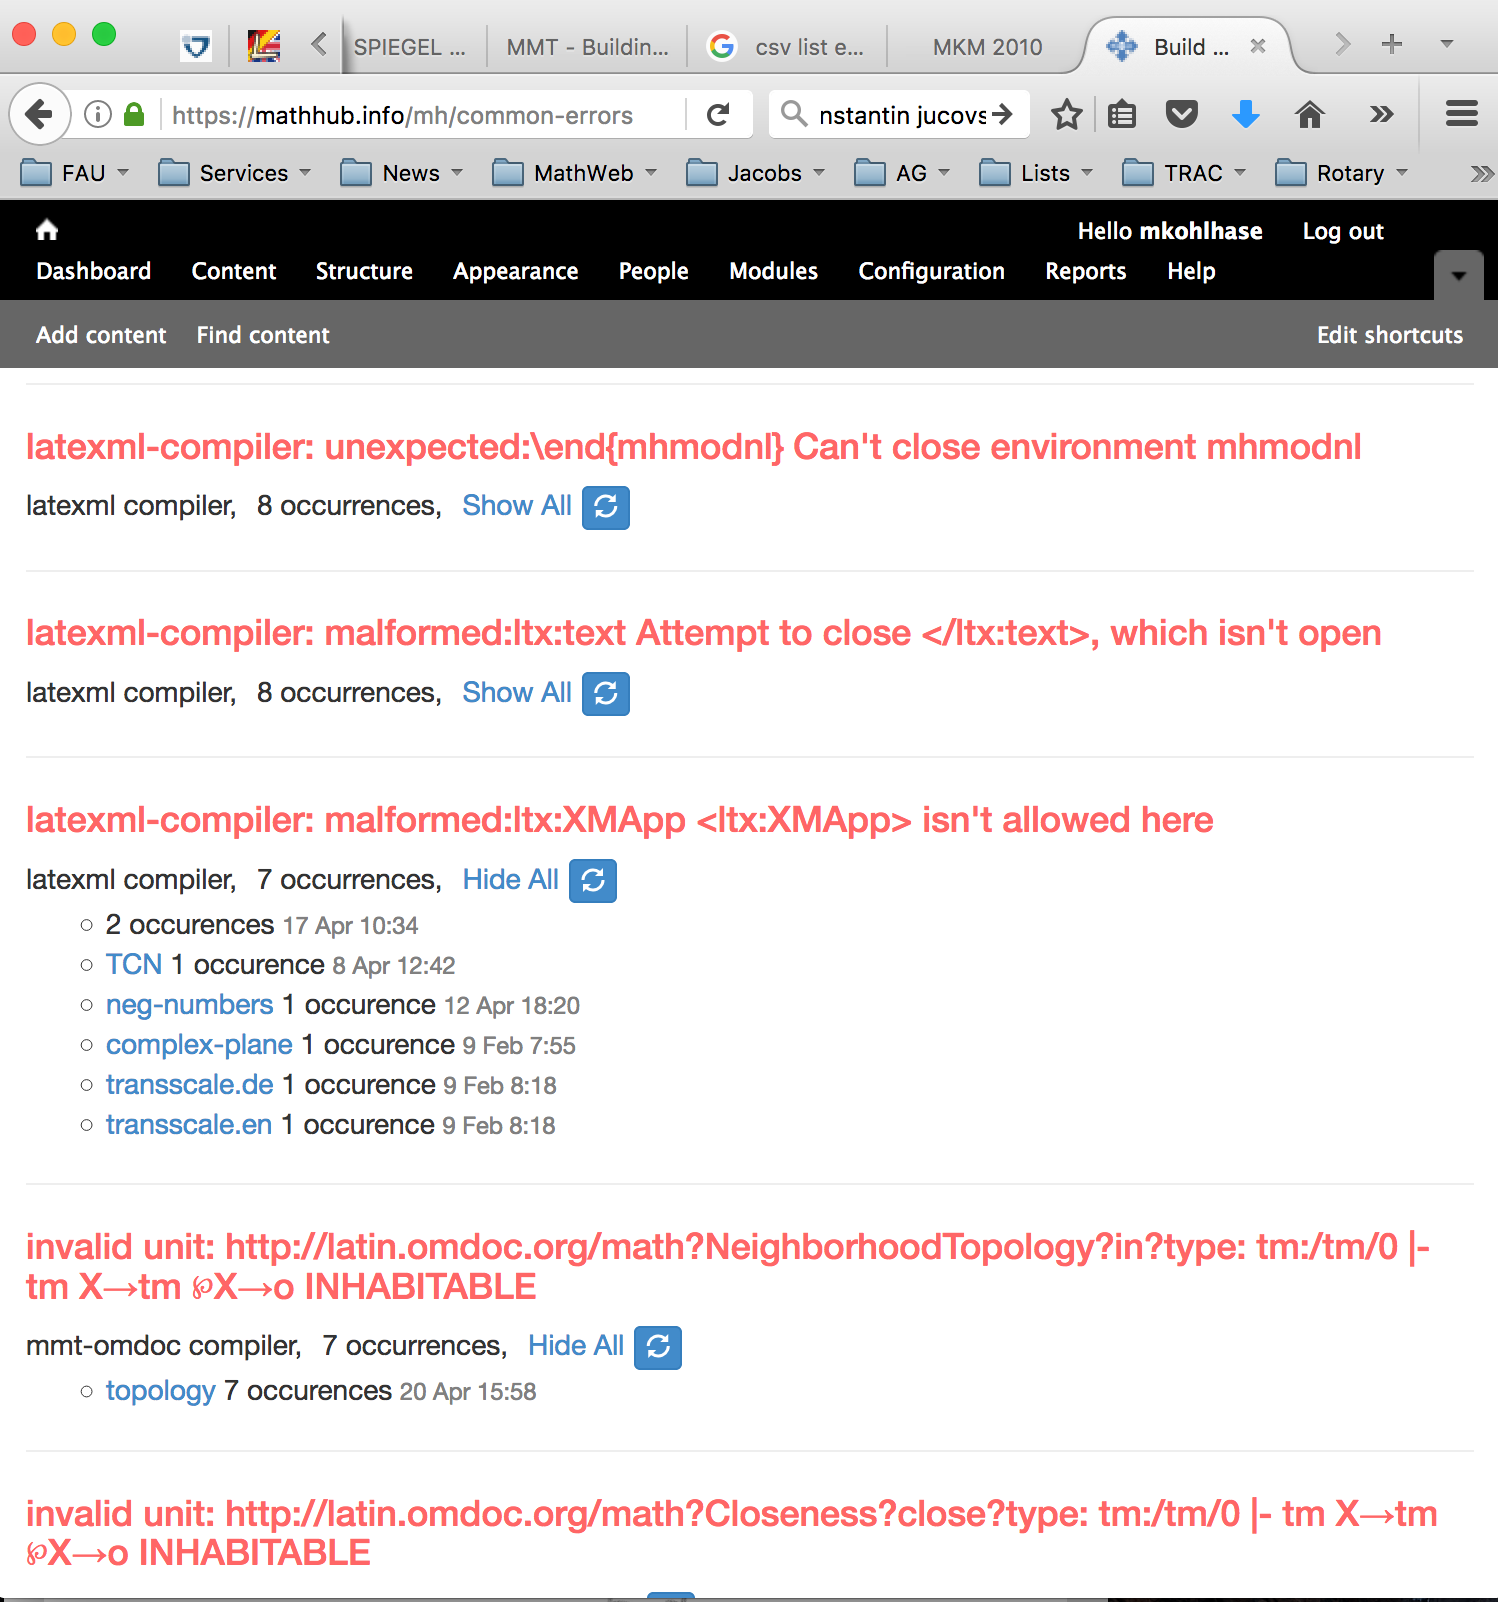
\includegraphics[width=12cm]{errorview}
  \caption{The \sys Error Viewer}\label{fig:errorview}
\end{figure}

In a second phase, the authors fully preload the documents semantically. In this phase,
the content is built into \omdoc/\mmt, loaded into the \mmt API and checked for semantic
link-consistency. In our experience the most important ``semantic editing service'' is to
track the errors encountered during these semantic checks. While it would be helpful to
have editor/IDE integration for the ensuing semantic debugging process, the main
advantage\footnote{This effect may however be partially caused by the fact that we
  currently still also have errors in the transformation pipeline, which necessitates full
  rebuilding of the \sys libraries interleaved with source debugging.}  can already be
reaped by a special, aggregating error viewer.  Figure~\ref{fig: errorview} shows a
fragment, where we see source errors (the first two) and error messages probably caused by
compiler problems. In both cases, the user can click on a the particular occurrences and
enter a web-based editing cycle which gives access to the logs and results of the
respective transformation steps. Any source errors can directly be fixed using the web
editing facilities (see~\ref{sec:web}).

\subsection{Local Editing Support for Formal Mathematics}\label{sec:local-formal}

Editing formal mathematical content poses a different set of challenges. As the content is
formal (i.e expressed in a formal language with well-defined semantics), its syntax and
semantics are fully machine-checkable, and this defines the standard of mathematical
quality. Consequently, an editing process that integrates syntax/semantics-checking --
which takes the form of type-checking in \mmt -- is needed for editing formal mathematics.

Figure~\ref{fig:jedit2} shows a JEdit-based IDE for \omdoc/\mmt content in \mmt surface
syntax that is tightly coupled with the \mmt API for semantic services;
see~\cite{Rabe:LII14} for details. In a nutshell, we can see the structural view of the
files in the panel on the left and the source file in the central pane. Both are
cross-linked for better structural and source navigation. In this example we also have a
type checking error in line 51 of the file \texttt{algebra.mmt}. It is indicated by the
red underline and the hovering the mouse over it gives the local error message, and the
error console at the bottom give additional details.

\begin{figure}[ht]\centering
  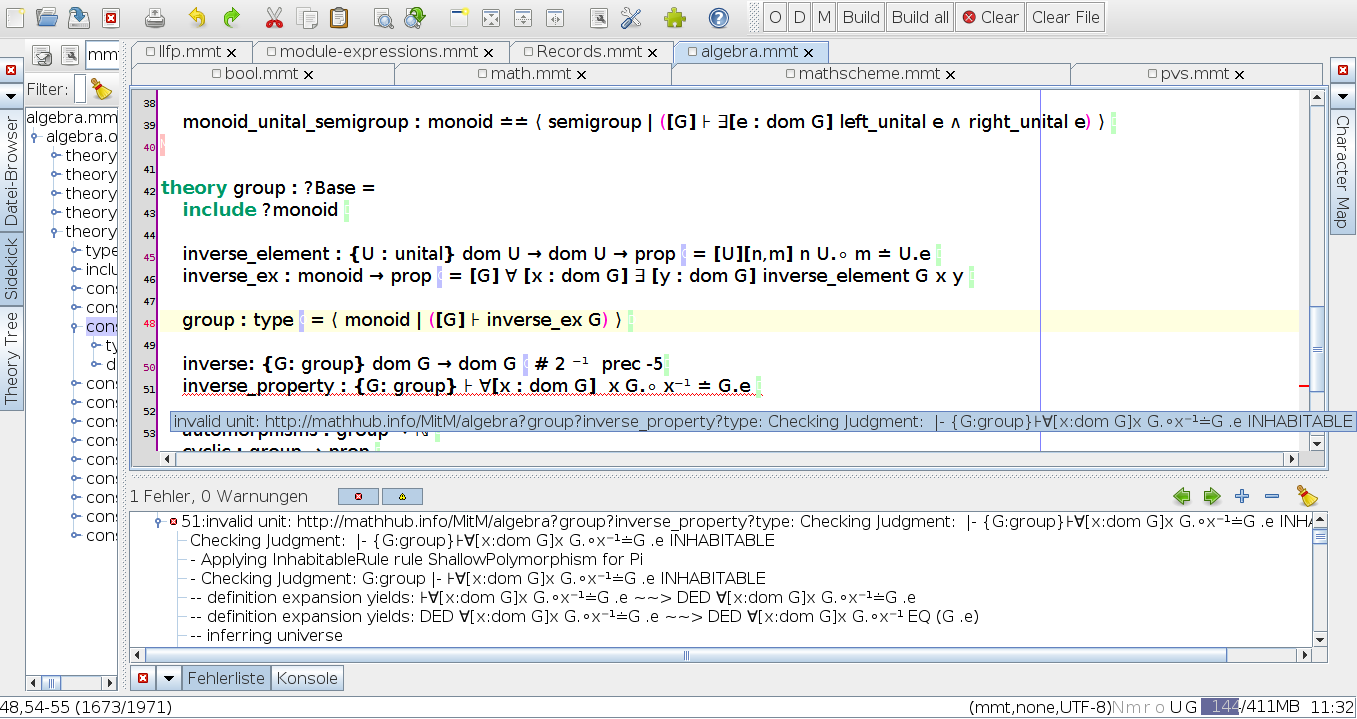
\includegraphics[width=15cm]{jedit2}
  \caption{Local Editing of \mmt Surface Syntax in JEdit}\label{fig:jedit2}
\end{figure}

In our experience, a dedicated, tightly integraded IDE is indispensible for the
development of formal mathematical content. This is analogous to the development of
software -- another form of formal content -- but for formal mathematical documents
type-checking -- which includes proof checking via the Curry-Howard isomorphism -- puts
even more semantic constraints on the edited material and thus an even heavier strain on
the author/maintainer.

\subsection{Web-based \sys Editing}\label{sec:web}

\begin{figure}[ht]\centering
  \fbox{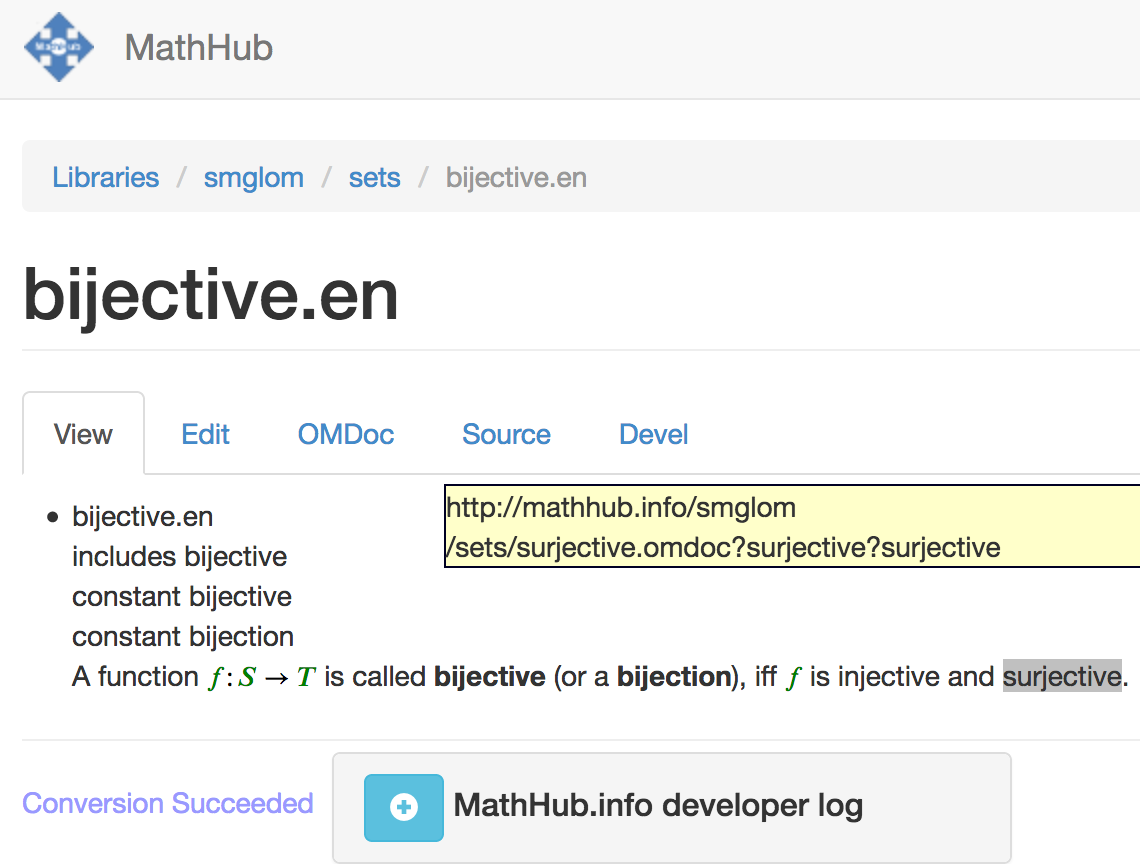
\includegraphics[width=8.5cm]{bijective}}\quad
  \fbox{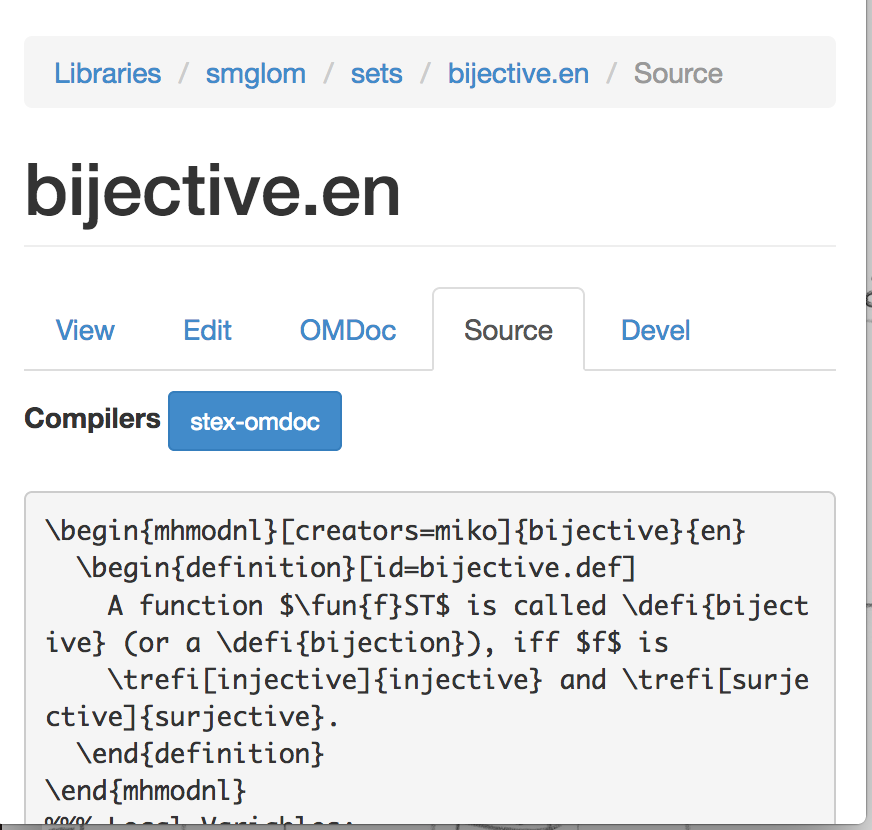
\includegraphics[width=6.5cm]{bijective-source}}
  \caption{Presentation and Source Views of A Glossary Entry}\label{fig:bijective}
\end{figure}

In the web-based workflows, we have the same requirements for integrating editing and
semantic correctness management as in the local workflows. In the current state of
development of \sys, we aim for a courser granularity of integration: we integrate at the
document level, which is commensurate with the fact that the quest for reusability in
active documents leads to small documents overall. Figure~\ref{fig:bijective} shows the
presentation of (the english language binding) of a glossary module for bijectivity. The
breadcrumbs at the top localize it in the \textsf{sets} archive in the \textsf{SMGloM}
library. The content presentation shows its dependencies and a human-oriented presentation
of the definition of bijectivity. There are five tabs with different forms of the same
content, the source view (expanded on the right of Figure~\ref{fig:bijective}), the
generated \omdoc, and an edit tab. The latter is just a link to the the corresponding
GitLab edit page; Figure~\ref{fig:bijective-edit}. 

\begin{figure}[ht]\centering
  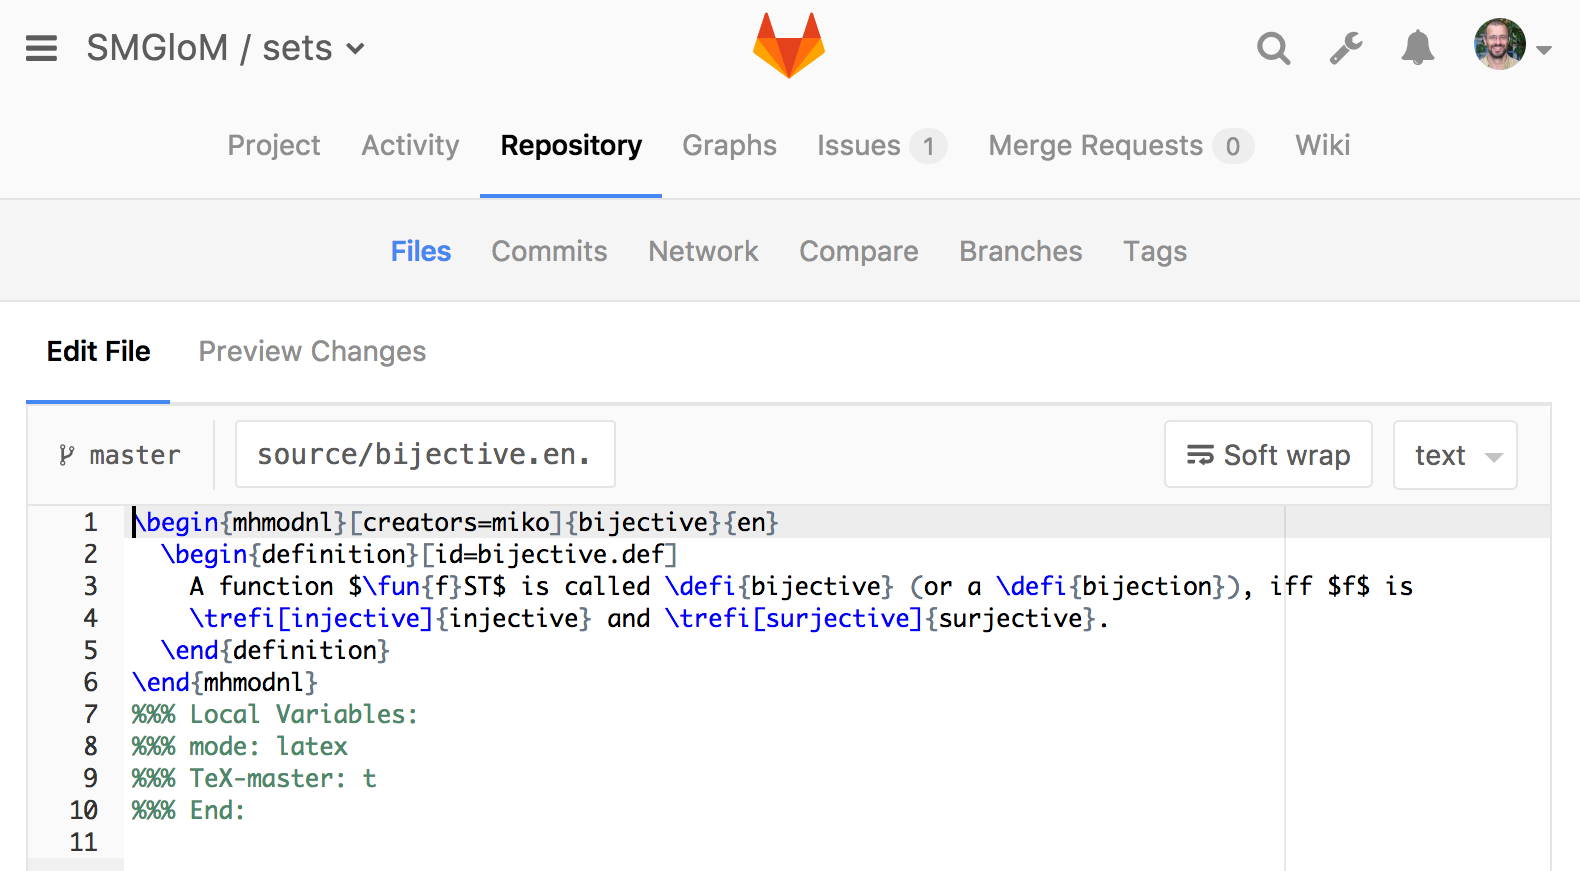
\includegraphics[width=10cm]{bijective-edit}
  \caption{Editing a Glossary Entry in GitLab}\label{fig:bijective-edit}
\end{figure}

This delegation is commensurate with the division of labor in the \sys system; GitLab
suports the full range of revision control interactions. In this case, users with
sufficient access rights can directly commit to the repository (and thus change the math
archive directly) users with less rights can directly initiate a pull request and submit
their changes to the archive maintainers in this way. 

But this delegation is not without technical challenges. An important concern is that the
user identities of the Drupal and GitLab instances have to be synchronized. Fortunately,
users can log into both systems with their GitHub account, which solves the problem at
least for the \pn project, where GitHub is universally emploayed and thus all partners
have GitHub accounts. Another problem is that GitLab only offers editing facilities for
files it considers text files, and it considers \mmt syntax files as binary, since they
contain lower ASCII symbols for component, declaration, and module separators.
Unfortunately, the media types are not configurable in GitLab, so we have to patch the
code. Building on an open-source system like GitLab and not the closed-source GitHub
allows to do that, but this still poses administration hassles with the fast-moving
release cycle of GitLab.

%%% Local Variables:
%%% mode: latex
%%% TeX-master: "report"
%%% End:

%  LocalWords:  sec:editing MitM:on DehKohKon:iop16,ODK-D6.2 ODKsysonto:on omdoc textbf
%  LocalWords:  GIT:on GitLab:on GitHub:on HorIacJuc:cscpnrr11 standardize ldots sec:lmh
%  LocalWords:  sec:web sec:surface optimized fig:arch lmh ocal lmh:on lmh-docker:on
%  LocalWords:  Formalized Kohlhase:ulsmf08 GinStaKoh:latexmldaemon11 JucKoh:sidesc10
%  LocalWords:  JucEth12:redsys centering includegraphics fig:errorview fig:jedit2 jedit2
%  LocalWords:  JEdit-based JEdit
\newpage
\section{Conclusion}\label{sec:concl}
We have surveyed the two document-formed user interfaces in the \pn project: Jupyter
Notebooks and Active Documents and developed a joint perspective on them that allows us to
propose a joint generalization oft the functionalities combines their respetive
advantages. We feel that embedding computations in arbitrary places in traditional
mathematical documents forms a natural generalization of the two existing user
interfaces. In particular the appearance as ``enhanced mathematical documents'' may make
the VRE more natural to mathematicians who have little experience with symbolic
computation tools, as they naturally have experiences with paper articles and textbooks
from their studies.

The survey and outlook provided by this report will be used as a basis for the discussion
of an integrated user interface and in the \pn project (WP4). As integration of knowledge
and computation (and interoperability between the various system involved) is a central
theme of WP6, this will require interaction between the work packages.

\subsection*{Acknowledgements} The authors are grateful to Min RK from Simula for
discussions on the inner workings of Jupyter and help with initial experiments with
setting up a a MMT kernel for Jupyter. Florian Rabe, Dan Alistarh, and Tom Wiesing have
worked on an initial integration of MMT with Jupyter that shaped and validated the vision
for an integrated user interface for the \pn VRE formulated in this report. Discussions
with Nicolas Thierry have refined the ideas presented here.

%%% Local Variables:
%%% mode: latex
%%% TeX-master: "report"
%%% End:
\newpage
\printbibliography
\end{document}

%%% Local Variables:
%%% mode: latex
%%% TeX-master: t
%%% End:

%  LocalWords:  maketitle githubissuedescription newpage tableofcontents newpage mathhub
%  LocalWords:  printbibliography
